\documentclass[a4paper, 12pt]{article}
\usepackage[top=2cm, bottom=2cm, left=1.5cm, right=1.5cm]{geometry}
\usepackage{graphicx}
\usepackage{float}
\usepackage{pgfplots}
\pgfplotsset{compat=1.18}
\usepackage{pgfplotstable}

\begin{document}
	\begin{center}
		Universidade Federal do Rio Grande do Norte
		
		Departamento de Engenharia da Computação e Automação
		
		DCA3703 - Programação Paralela
		
		\textbf{Tarefa 5 - Comparação entre programação sequencial e paralela}
		
		\textbf{Aluno:} Daniel Bruno Trindade da Silva
	\end{center}
	
	\section{Introdução}
	\hspace{.7cm}Nesta prática, buscamos comparar a programação paralela com a sequencial, para isso desenvolvemos um programa capaz de contar quantos números primos existem entre 2 e um dado \textit{n} e o implementamos em uma versão sequencial e outra paralela, mantendo a lógica original do programa para garantir uma comparação justa de desempenho. Por fim comparamos o desempenho das versões do código para entender o impacto da paralelização no tempo de execução.
	
	\section{Metodologia}
	\hspace{.7cm}Para a versão de execução sequencial, implementamos o código com uma  função chamada \texttt{ehPrimo()} que recebe um número e retorna \texttt{true} caso seja primo, \texttt{false} caso não:
	
	\begin{verbatim}
		bool ehPrimo(int num) {
			   if (num < 2) return false;
			   for (int i = 2; i * i <= num; i++) {
				      if (num % i == 0) return false;
			   }
			   return true;
		}
	\end{verbatim}
	
	Na \texttt{main()} foi implementado um laço de repetição que passa por todos os inteiros de 2 a \textit{n} testando o valor com a função \texttt{ehPrimo()}. Nesse caso temos dois laços de repetição aninhados que testam os números um a um.
	
	\begin{verbatim}
		int main() {
		    int contador = 0;
		    struct timeval inicio, fim;
		    double time_lapsed;
		    gettimeofday(&inicio, NULL);
		    for (int i = 2; i <= N; i++) {
		        if (ehPrimo(i)) {
		            contador++;
		        }
		    }
		    
		    gettimeofday(&fim, NULL); 
		    time_lapsed = get_time(inicio, fim);
		    printf("Quantidade de números primos eh: %d\n", contador);
		    printf("Tempo gasto: %f segundos\n", time_lapsed);
		    
		    return 0;
		}
	\end{verbatim}
	
	Para a versão do código paralela, mantivemos a lógica da versão sequencial, porém acrescentamos a diretiva \texttt{\#pragma omp parallel for} que paraleliza a execução do laço de repetição, distribuindo entre os threads disponíveis. Devido a condição de corrida estabelecida pelo paralelismo do laço precisamos adicionar uma área crítica na variável contador, e nesse caso adicionamos a diretiva \texttt{reduction(+:contador)} que protege a variável desse problema. CCom as alterações necessárias, a função \texttt{main()} ficou da seguinte forma:
	
	\begin{verbatim}
		int main() {
		    int contador = 0;
		    struct timeval inicio, fim;
		    double time_lapsed;
		    gettimeofday(&inicio, NULL);
		    
		    #pragma omp parallel for reduction(+:contador)
		    
		    for (int i = 2; i <= N; i++) {
		        if (ehPrimo(i)) {
		            contador++;
		        }
		    }
			
		    gettimeofday(&fim, NULL); 
		    time_lapsed = get_time(inicio, fim);
		    printf("Quantidade de números primos eh: %d\n", contador);
		    printf("Tempo gasto: %f segundos\n", time_lapsed);
			
		    return 0;
		}
	\end{verbatim}
	
	
	Em ambas as versões o tempo de execução foi calculado utilizando a função \texttt{gettimeofday()} da biblioteca \texttt{sys/time.h} para que possamos comparar seus resultados.
	
	\section{Resultados}
	Vamos realizar a comparação dos tempos de execução de cada uma das versões do código:
	
	
	\begin{center}
		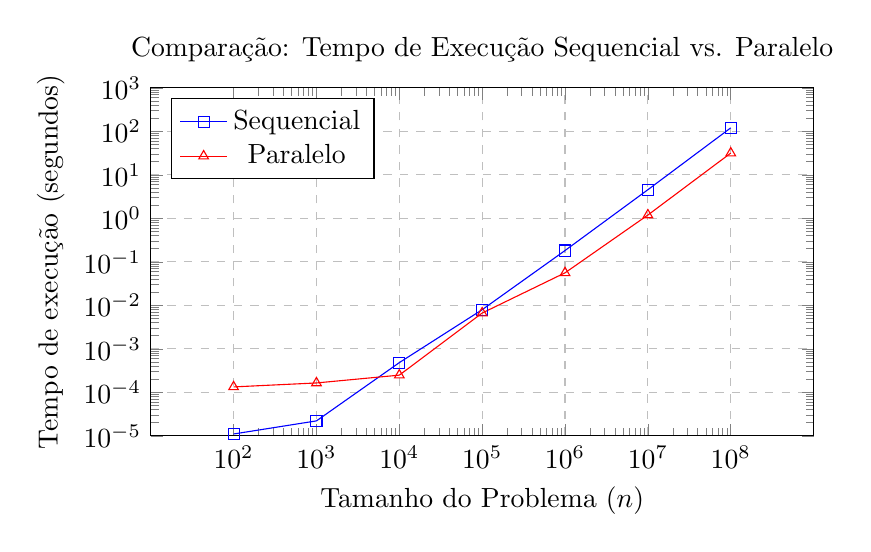
\begin{tikzpicture}
			\begin{loglogaxis}[
				title={Comparação: Tempo de Execução Sequencial vs. Paralelo},
				xlabel={Tamanho do Problema ($n$)},
				ylabel={Tempo de execução (segundos)},
				xmin=1e1, xmax=1e9,
				ymin=1e-5, ymax=1e3,
				xtick={1e2,1e3,1e4,1e5,1e6,1e7,1e8},
				xticklabels={$10^2$,$10^3$,$10^4$,$10^5$,$10^6$,$10^7$,$10^8$},
				ytick={1e-5,1e-4,1e-3,1e-2,1e-1,1e0,1e1,1e2,1e3},
				ymajorgrids=true,
				xmajorgrids=true,
				grid style=dashed,
				legend pos=north west,
				width=10cm,
				height=6cm
				]
				
				% Dados sequenciais
				\addplot[color=blue, mark=square]
				coordinates {
					(100, 0.000011)
					(1000, 0.000022)
					(10000, 0.000481)
					(100000, 0.007936)
					(1000000, 0.181999)
					(10000000, 4.555114)
					(100000000, 120.311929)
				};
				\addlegendentry{Sequencial}
				
				% Dados paralelos
				\addplot[color=red, mark=triangle]
				coordinates {
					(100, 0.000133)
					(1000, 0.000164)
					(10000, 0.000248)
					(100000, 0.006644)
					(1000000, 0.055840)
					(10000000, 1.191834)
					(100000000, 31.657761)
				};
				\addlegendentry{Paralelo}
				

				\addlegendentry{$O(n)$}
				
			\end{loglogaxis}
		\end{tikzpicture}
	\end{center}
	
	\begin{center}
		% Gráfico de Speedup (ganho de desempenho)
		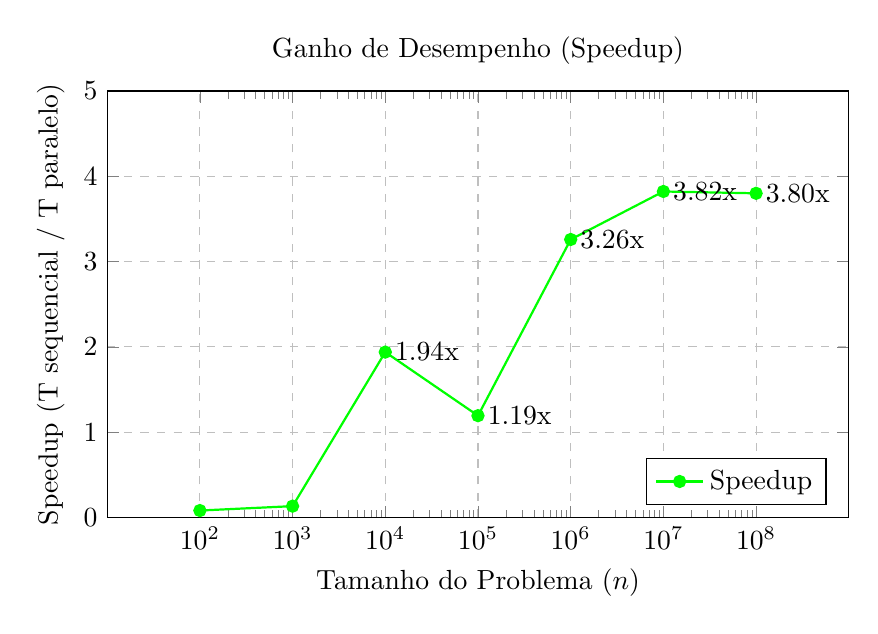
\begin{tikzpicture}
			\begin{semilogxaxis}[
				title={Ganho de Desempenho (Speedup)},
				xlabel={Tamanho do Problema ($n$)},
				ylabel={Speedup (T sequencial / T paralelo)},
				xmin=1e1, xmax=1e9,
				ymin=0, ymax=5,
				xtick={1e2,1e3,1e4,1e5,1e6,1e7,1e8},
				xticklabels={$10^2$,$10^3$,$10^4$,$10^5$,$10^6$,$10^7$,$10^8$},
				ymajorgrids=true,
				xmajorgrids=true,
				grid style=dashed,
				legend pos=south east,
				width=11cm,
				height=7cm,
				ytick={0,1,2,3,4,5},
				yticklabels={0,1,2,3,4,5}
				]
				
				% Cálculo do speedup
				\addplot[color=green, mark=*, thick]
				coordinates {
					(100, 0.000011/0.000133)
					(1000, 0.000022/0.000164)
					(10000, 0.000481/0.000248)
					(100000, 0.007936/0.006644)
					(1000000, 0.181999/0.055840)
					(10000000, 4.555114/1.191834)
					(100000000, 120.311929/31.657761)
				};
				\addlegendentry{Speedup}
				
				% Anotações com valores de speedup
				\node[anchor=west] at (axis cs:1e4,1.94) {1.94x};
				\node[anchor=west] at (axis cs:1e5,1.19) {1.19x};
				\node[anchor=west] at (axis cs:1e6,3.26) {3.26x};
				\node[anchor=west] at (axis cs:1e7,3.82) {3.82x};
				\node[anchor=west] at (axis cs:1e8,3.80) {3.80x};
				
			\end{semilogxaxis}
		\end{tikzpicture}
	\end{center}
	
	Com isso, podemos observar que, para valores pequenos de \textit{n} (até 10.000), a versão paralela apresenta desempenho igual ou inferior ao da versão sequencial. Isso ocorre porque a criação, gerenciamento e sincronização das threads introduzem um custo computacional adicional, conhecido como \textit{overhead}, que não compensa o paralelismo nesse intervalo. No entanto, para valores maiores (acima de 100.000), a versão paralela começa a superar a execução sequencial, alcançando uma melhoria de desempenho de até 3,8 vezes na execução da tarefa.
	
	\section{Conclusão}
	\hspace{0.7cm}A comparação entre as abordagens sequencial e paralela demonstrou que, para tarefas computacionalmente simples ou com baixo volume de dados, a paralelização pode não trazer benefícios devido ao overhead de gerenciamento das threads. Entretanto, conforme o tamanho do problema aumenta, os ganhos de desempenho se tornam significativos, alcançando um speedup de até 3,8 vezes em nossa análise. Essa prática evidencia a importância da escolha criteriosa da abordagem de programação, considerando o custo-benefício do paralelismo.
	
	
\end{document}